\documentclass[aspectratio=169]{beamer}

\usetheme{default}
\usecolortheme{seahorse}
\setbeamertemplate{navigation symbols}{}
\setbeamertemplate{footline}[frame number]

\usepackage{amsmath,amssymb}
\usepackage{mathtools}
\usepackage{graphicx}

\newcommand{\R}{\mathbb{R}}
\newcommand{\norm}[1]{\lVert #1 \rVert}

\title{Finding Principal Directions}
\subtitle{Mathematics of Machine Learning}
\author{Math 3180 --- University of Connecticut}
\date{}

\begin{document}

\begin{frame}
  \titlepage
\end{frame}

%------------------------------------------------------------------
\begin{frame}{The Data Matrix}
  \begin{itemize}
    \item $X$ is an $N \times k$ matrix:
      \begin{itemize}
        \item rows $\longleftrightarrow$ samples
        \item columns $\longleftrightarrow$ features
      \end{itemize}
    \medskip
    \item \textbf{Assumption:} the data is \emph{centered} ---
      each column sums to zero.
    \medskip
    \item Each row of $X$ is a point in $\R^{k}$.\\
      The $N$ rows form a \emph{cloud of points} in $\R^{k}$.
  \end{itemize}
\end{frame}

%------------------------------------------------------------------
\begin{frame}{Variance in a Direction}
  \begin{columns}[T]
    \begin{column}{0.52\textwidth}
      \begin{itemize}
        \item Let $u \in \R^{k}$ be a \textbf{unit vector}, $\norm{u}^{2}=1$.
        \medskip
        \item The \emph{variance of the data in direction $u$} is
          \[
            \sigma_{u}^{2} \;=\; u^{T} D_{0}\, u,
          \]
          where $D_{0} = \dfrac{1}{N} X^{T} X$ is the \textbf{covariance matrix}.
        \medskip
        \item $\sigma_{u}^{2} = \dfrac{1}{N}\displaystyle\sum_{i=1}^{N}(x_{i}\cdot u)^{2}$
          is the mean squared projection onto $u$.
      \end{itemize}
    \end{column}
    \begin{column}{0.46\textwidth}
      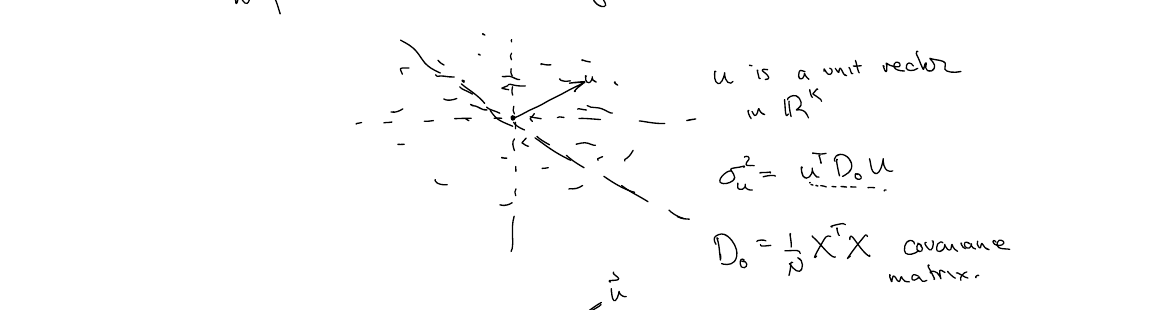
\includegraphics[width=\textwidth]{sketch_cloud.png}
    \end{column}
  \end{columns}
\end{frame}

%------------------------------------------------------------------
\begin{frame}{The Optimization Problem}
  \begin{columns}[T]
    \begin{column}{0.58\textwidth}
      \begin{block}{Goal}
        Find the unit vector $u \in \R^{k}$ that \textbf{maximizes}
        $\sigma_{u}^{2} = u^{T} D_{0}\, u$.
      \end{block}

      \bigskip
      \begin{itemize}
        \item This is a \emph{constrained} optimization problem:
          \[
            \text{maximize } u^{T}D_{0}u
            \quad \text{s.t.} \quad \norm{u}^{2} = 1.
          \]
        \item Tool: \textbf{Lagrange multipliers}.
      \end{itemize}
    \end{column}
    \begin{column}{0.38\textwidth}
      \vspace{1em}
      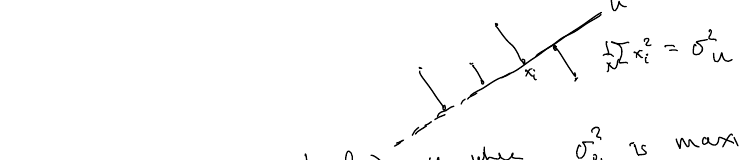
\includegraphics[width=\textwidth]{sketch_projection.png}
      \smallskip

      \footnotesize Projections $x_i \cdot u$ of data points onto $u$;
      their mean square is $\sigma_u^2$.
    \end{column}
  \end{columns}
\end{frame}

%------------------------------------------------------------------
\begin{frame}{Lagrange Multipliers: General Setup}
  \begin{itemize}
    \item \textbf{Objective}: $F(x_{1},\ldots,x_{k})$ --- the function to maximize.
    \item \textbf{Constraint}: $g(x_{1},\ldots,x_{k}) = 0$.
  \end{itemize}

  \medskip
  Form the \textbf{Lagrangian}:
  \[
    S(x_{1},\ldots,x_{k},\lambda) \;=\; F - \lambda\, g.
  \]

  \medskip
  Critical points satisfy:
  \[
    \frac{\partial S}{\partial x_{i}} = 0 \quad (i=1,\ldots,k)
    \qquad \text{and} \qquad
    \frac{\partial S}{\partial \lambda} = 0 \;\Longleftrightarrow\; g = 0.
  \]
\end{frame}

%------------------------------------------------------------------
\begin{frame}{Setting Up the Lagrangian}
  Write $D_{0} = (d_{ij})$.  Then
  \[
    \sigma_{u}^{2} \;=\; u^{T}D_{0}u
    \;=\; \sum_{r=1}^{k}\sum_{s=1}^{k} u_{r}\,d_{rs}\,u_{s}.
  \]

  \medskip
  The constraint is $g(u) = u_{1}^{2}+\cdots+u_{k}^{2}-1 = 0$.

  \medskip
  The Lagrangian is:
  \[
    S(u,\lambda)
    \;=\; \sum_{r=1}^{k}\sum_{s=1}^{k} u_{r}\,d_{rs}\,u_{s}
    \;-\; \lambda\!\left(u_{1}^{2}+\cdots+u_{k}^{2}-1\right).
  \]
\end{frame}

%------------------------------------------------------------------
\begin{frame}{Computing the Partial Derivatives}
  Differentiating $S$ with respect to $u_{i}$ and using the symmetry
  $d_{rs} = d_{sr}$ of $D_{0}$:
  \[
    \frac{\partial S}{\partial u_{i}}
    \;=\; 2\sum_{s=1}^{k} d_{is}\,u_{s} \;-\; 2\lambda u_{i}.
  \]

  \medskip
  In vector form:
  \[
    \nabla_{u} S
    \;=\; 2\,D_{0}\,u \;-\; 2\lambda\,u
    \;=\; 2\,(D_{0} - \lambda I)\,u.
  \]

  \medskip
  The condition $\dfrac{\partial S}{\partial\lambda}=0$ gives $\norm{u}^{2}=1$.
\end{frame}

%------------------------------------------------------------------
\begin{frame}{The Critical Point Equations}
  Setting $\nabla_{u} S = 0$ and $\partial S/\partial\lambda = 0$ gives
  the system:
  \[
    \begin{cases}
      (D_{0} - \lambda I)\,u = 0, \\[4pt]
      \norm{u}^{2} = 1.
    \end{cases}
  \]

  \medskip
  The first equation is equivalent to
  \[
    \boxed{D_{0}\,u = \lambda\,u.}
  \]

  \bigskip
  \begin{center}
    \textbf{$u$ is an eigenvector of $D_{0}$ with eigenvalue $\lambda$,
    normalized so that $\norm{u}=1$.}
  \end{center}
\end{frame}

%------------------------------------------------------------------
\begin{frame}{The Value of $\sigma_{u}^{2}$ at a Critical Point}
  If $D_{0}u = \lambda u$ and $\norm{u}=1$, then
  \[
    \sigma_{u}^{2}
    \;=\; u^{T}D_{0}u
    \;=\; u^{T}(\lambda u)
    \;=\; \lambda\,\norm{u}^{2}
    \;=\; \lambda.
  \]

  \medskip
  The variance in direction $u$ \emph{equals} the corresponding eigenvalue.
\end{frame}

%------------------------------------------------------------------
\begin{frame}{Main Theorem}
  \begin{theorem}
    The critical points of $\sigma_{u}^{2} = u^{T}D_{0}u$ subject to
    $\norm{u}^{2}=1$ are exactly the unit eigenvectors of $D_{0}$.
    At such a critical point, $\sigma_{u}^{2} = \lambda$ (the
    corresponding eigenvalue).
  \end{theorem}

  \bigskip
  \begin{itemize}
    \item The \textbf{maximum variance} equals the \textbf{largest eigenvalue}
      of $D_{0}$; it is achieved along the corresponding eigenvector.
    \item The \textbf{minimum variance} equals the \textbf{smallest eigenvalue}
      of $D_{0}$.
  \end{itemize}

  \bigskip
  \begin{block}{Fact}
    $D_{0} = \tfrac{1}{N}X^{T}X$ is symmetric, so all its eigenvalues
    are real (and in fact non-negative).
  \end{block}
\end{frame}

\end{document}
